\Exercise Expressa en forma polar cadascun dels punts següents:

\begin{multicols}{2}
  \begin{enumerate}
    \item $(3,3)$  \item $(-\sqrt{3},3)$ \item $(-\sqrt{8},-\sqrt{8})$ \item $(6,-8)$
  \end{enumerate}
\end{multicols}

\Answer

D'acord amb la imatge, el canvi de coordenades cartesianes a polars ve donada per:


\begin{minipage}{0.49\linewidth}
  \begin{center}  
    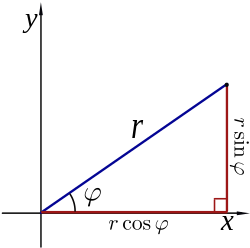
\includegraphics[scale=0.5]{polar_fig}
  \end{center}
\end{minipage}
\hspace{0.01\linewidth}
\begin{minipage}{0.49\linewidth}
  \[\begin{cases}r=\sqrt{x^2+y^2}\\ \varphi=\atan{\frac{y}{x}}\end{cases}\]
\end{minipage}
Per tant:
\begin{enumerate}
  \item \[\begin{cases}r=\sqrt{3^2+3^2}=3\sqrt{2}\\\varphi=\atan{1}=\frac{\pi}{4}\end{cases}\]  
  \item  \[\begin{cases}r=\sqrt{{-\sqrt{3}}^2+3^2}=2\sqrt{3}\\\varphi=\atan{-\frac{3}{\sqrt{3}}}=\frac{2\pi}{3}\end{cases}\]  
  \item \[\begin{cases}r=\sqrt{-\sqrt{8}^2+-\sqrt{8}^2}=4\\\varphi=\atan{\frac{-\sqrt{8}}{-\sqrt{8}}}=-\frac{5\pi}{4}\end{cases}\]  
  \item \[\begin{cases}r=\sqrt{6^2+(-8)^2}=10\\\varphi=\atan{\frac{-8}{6}}=2.21\, \mathrm{rad}\end{cases}\]  
\end{enumerate}
\begin{center}
  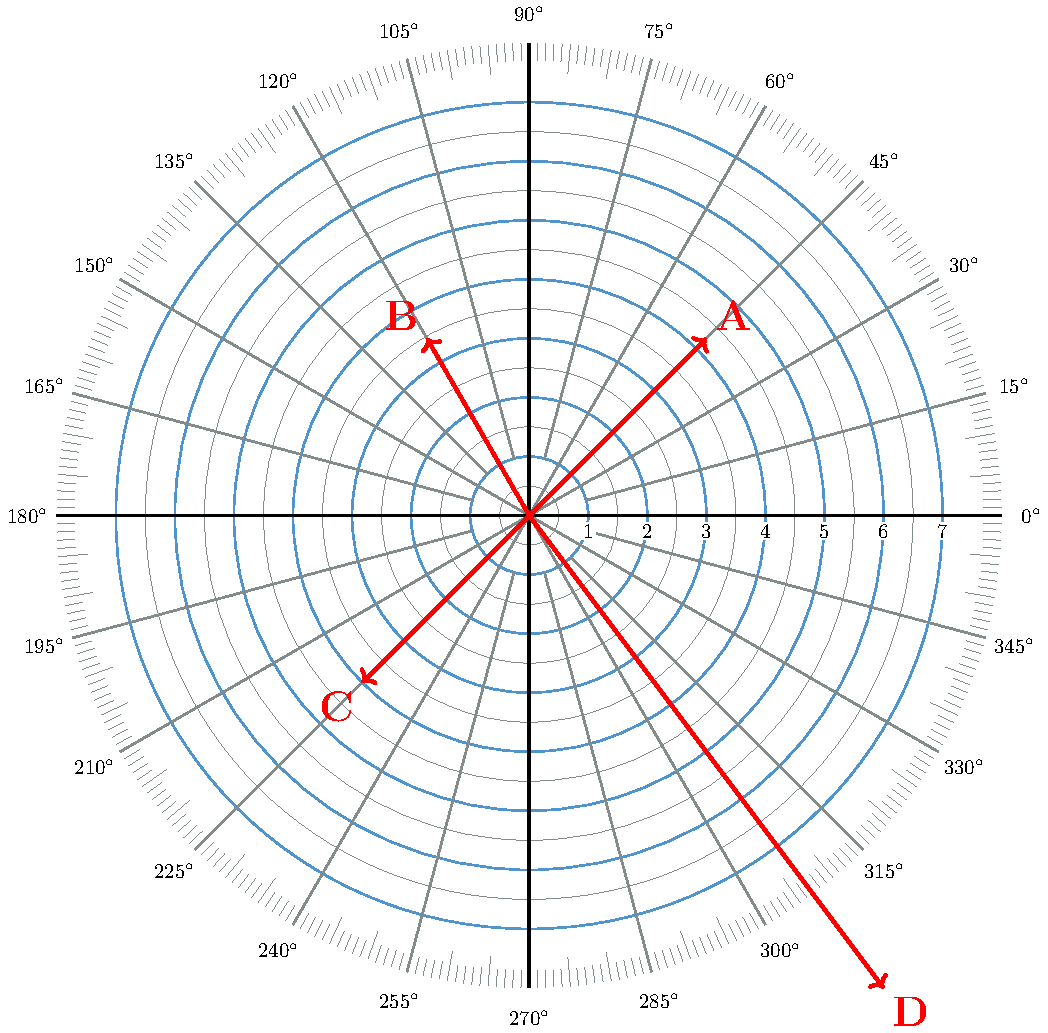
\includegraphics[scale=0.6]{polar1}
\end{center}

\blacksquare 